% Bagian Tahapan Percobaan
\section*{Tahapan Percobaan} % Jika ada tahapan percobaan

Dalam modul ini, sebelum melakukan konfigurasi routing statis dan dinamis, terlebih dahulu kita harus menyiapkan topologi yang akan digunakan untuk percobaan 1 dan 2. Topologi yang digunakan ditulis dalam kertas seperti pada Gambar \ref{fig:topo}.

\begin{figure}[H]
    \centering
    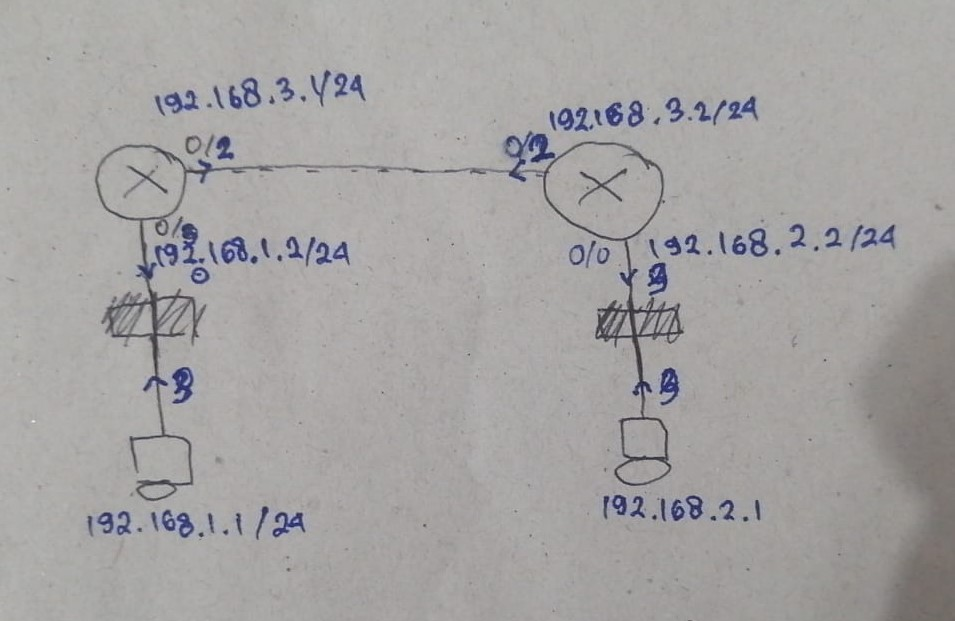
\includegraphics[width=0.8\textwidth]{img/topologi.jpeg}
    \caption{Topologi yang akan digunakan}
    \label{fig:topo}
\end{figure}

Setelah topologi selesai disiapkan, langkah selanjutnya adalah melakukan konfigurasi routing statis dan dinamis pada perangkat MikroTik. Berikut adalah tahapan percobaan yang harus dilakukan:

\subsection*{Percobaan 1: Konfigurasi Static Routing}

\begin{enumerate}
    \item \textbf{Buka WinBox dan Sambungkan ke Router:}
    \begin{enumerate}
        \item Buka aplikasi WinBox di PC1.
        \item Klik \texttt{Neighbors}, lalu klik \texttt{Refresh}.
        \item Klik dua kali router yang terdeteksi, lalu klik \texttt{Connect}.
    \end{enumerate}
    
    \item \textbf{Atur IP Address Router 1:}
    \begin{enumerate}
        \item Pada tab \texttt{IP > Addresses}, masukkan IP Address untuk interface \texttt{ether2} dan \texttt{ether4}.
        \item Pastikan IP Address berbeda dari contoh di modul dan sesuai aturan.
    \end{enumerate}
    
    \item \textbf{Konfigurasi Routing Statis Router 1:}
    \begin{enumerate}
        \item Buka tab \texttt{IP > Routes}.
        \item Tambahkan jaringan dengan memasukkan alamat jaringan tujuan dan alamat Gateway \texttt{router2}.
    \end{enumerate}
    
    \item \textbf{Atur IP Address Router 2:}
    \begin{enumerate}
        \item Buka WinBox dan sambungkan ke \texttt{Router2}.
        \item Pada tab \texttt{IP > Addresses}, masukkan IP Address untuk interface \texttt{ether2} dan \texttt{ether4}.
        \item Pastikan IP Address berbeda dari contoh di modul dan sesuai aturan.
    \end{enumerate}
    
    \item \textbf{Konfigurasi Routing Statis Router 2:}
    \begin{enumerate}
        \item Buka tab \texttt{IP > Routes}.
        \item Tambahkan jaringan dengan memasukkan alamat jaringan tujuan dan alamat Gateway \texttt{router1}.
    \end{enumerate}
    
    \item \textbf{Uji Koneksi:}
    \begin{enumerate}
        \item Lakukan tes ping dari \texttt{PC1} ke \texttt{router2}.
        \item Lakukan tes ping dari \texttt{PC2} ke \texttt{router1}.
        \item Jika status menunjukkan \texttt{terhubung}, maka percobaan berhasil.
    \end{enumerate}
\end{enumerate}

\subsection*{Percobaan 2: Konfigurasi Dynamic Routing}

\subsubsection*{Konfigurasi Router 1}

\begin{enumerate}
    \item \textbf{Buka WinBox}: Buka aplikasi WinBox dan lakukan koneksi ke Router 1.
    \item \textbf{Atur IP Address}: Berikan IP Address pada interface \texttt{ether} (yang terhubung ke laptop/PC) dan \texttt{ether} (yang terhubung ke Router lain) pada tab \texttt{IP > Addresses}. Pastikan IP Address yang diberikan sesuai dan berbeda dari contoh di modul.
    \item \textbf{Routing Dinamis (RIP)}:
    \begin{enumerate}
        \item Buka tab \texttt{Routing > RIP}.
        \item Pada bagian \texttt{Interfaces}, tambahkan interface baru dan atur interface menjadi \texttt{ether} (yang terhubung ke Router lain).
        \item Pada bagian \texttt{Networks}, tambahkan dua network baru:
        \begin{itemize}
            \item Network antara PC1 dengan Router 1.
            \item Network antara Router 1 dengan Router 2.
        \end{itemize}
        \item Pada bagian \texttt{Neighbours}, tambahkan alamat IP Router 2.
    \end{enumerate}
\end{enumerate}

\subsubsection*{Konfigurasi Router 2}

\begin{enumerate}
    \item \textbf{Buka WinBox}: Buka aplikasi WinBox dan lakukan koneksi ke Router 2.
    \item \textbf{Atur IP Address}: Berikan IP Address pada interface \texttt{ether} (yang terhubung ke laptop/PC) dan \texttt{ether} (yang terhubung ke Router lain) pada tab \texttt{IP > Addresses}. Pastikan IP Address yang diberikan sesuai dan berbeda dari contoh di modul.
    \item \textbf{Routing Dinamis (RIP)}:
    \begin{enumerate}
        \item Buka tab \texttt{Routing > RIP}.
        \item Pada bagian \texttt{Interfaces}, tambahkan interface baru dan atur interface menjadi \texttt{ether} (yang terhubung ke Router lain).
        \item Pada bagian \texttt{Networks}, tambahkan dua network baru:
        \begin{itemize}
            \item Network antara PC2 dengan Router 2.
            \item Network antara Router 1 dengan Router 2.
        \end{itemize}
        \item Pada bagian \texttt{Neighbours}, tambahkan alamat IP Router 1.
    \end{enumerate}
\end{enumerate}

\subsubsection*{Pengujian Konfigurasi}

\begin{enumerate}
    \item \textbf{Ping Router 1 ke Router 2}: Lakukan tes ping dari Router 1 ke Router 2 untuk memastikan konektivitas.
    \item \textbf{Ping Router 2 ke Router 1}: Lakukan tes ping dari Router 2 ke Router 1 untuk memastikan konektivitas.
\end{enumerate}